\documentclass[11pt,a4paper,twoside,graphicx,color]{article}
%
\usepackage[margin=2cm]{geometry}
\usepackage[margin=2cm]{geometry}
\usepackage[pdftex]{graphicx}
\usepackage{color}
\usepackage{txfonts}
\usepackage{paralist}
\usepackage[numbers]{natbib}
\setlength{\bibsep}{0.0pt}
\usepackage{amssymb}
\usepackage[breaklinks, colorlinks, citecolor=blue, linkcolor=MyBlue, urlcolor=RoyalPurple, colorlinks=true, linkcolor=blue, debug, baseurl=' ']{hyperref}
%
\textheight 260mm
\textwidth 178mm
\oddsidemargin -8mm
\evensidemargin -8mm
\marginparwidth 50pt
\topmargin -22mm
\brokenpenalty=10000
\sloppy
%
\bibpunct{(}{)}{;}{a}{}{,} 
\bibliographystyle{aa}

%%%%%%%%%%%%%%%%%%%%%%%%%%%%%%%%%%%%%%%%%%%%%%%%
\begin{document}
%\section{Abstract}
%We propose to observe two of the Planck SZ discovered clusters of galaxies as a pilot project to test the feasibility of lensing studies with the GTC. The targets are PSZ1~G046.13+30.75 and PSZ1~G045.85+57.71, which have already been followed-up by XMM X-ray observations and high resolution Sunyaev-Zel'dovich observation with NIKA+IRAM30m. The same clusters are also part of an XMM program, and we then also dispose of high-quality X-ray data for them. The tSZ and X-ray signals probe the diffuse baryonic gas component of galaxy clusters. Under the hypothesis of hydrostatic equilibrium, we can use these baryonic tracer to recover the cluster total mass. Through gravitational lensing we can instead directly explore the distribution of the dark matter component, which largely dominates the cluster total mass. The goal of this proposal is then to test the GTC lensing capabilities, and the complementarity with NIKA observations, in view of the NIKA2 large program aiming at observing 50 objects, to explore the properties of the cluster population beyond the local Universe (z $>$ 0.5). The complementarity of the tSZ and gravitational lensing can in fact allow studying how does the distribution both dark matter and gas evolve with redshift and the complex interplay between the gravitational and non-gravitational processes governing the cluster astrophysics.

%%%%%%%%%%%%%%%%%%%%%%%%%%%%%%%%%%%%%%%%%%%%%%%%
\section{Scientific context}
%========== Clusters cosmology: cluster assembly and open questions
%\paragraph{\large The hierarchical formation of galaxy clusters}
Clusters of galaxies provide valuable information concerning the formation of large scale structures. Their number density as a function of mass and redshift is particularly sensitive to the expansion history and the growth of structures in the Universe \citep[see e.g.]{allen2011}. Therefore they represent a valuable tool for cosmology. The observable properties of clusters reflect their formation through hierarchical gravitational collapse, by accretion and merging of smaller sub-clusters and groups, as well as the contribution of non-gravitational processes (e.g. AGN feedback and supernova-driven galactic winds) that can affect their observed properties to a large extent \citep[e.g.][]{sembolini2014}. Consequently, a detailed characterization of the assembly of the dark (mainly governed by gravity) and the baryonic (governed by both gravity and radiative processes) matter components, as well as the interplay between the two, is mandatory to control the impact of cluster astrophysics on their observable properties, which in turn affects any cosmological interpretation. At present, cluster derived cosmological constraints are limited by our incomplete knowledge of cluster physics, which turns out into astrophysical systematics, such as those affecting the clusters mass reconstruction, performed through baryonic proxies from X-ray and Sunyaev-Zel'dovich (SZ) observables \citep[e.g. ][]{planck_nc_2015}.

%========== Clusters cosmology: cluster assembly and open questions
\paragraph{\large Probing the co-evolution of the baryonic and the dark matter components}
The co-evolution of the dark and the baryonic matter can be probed from resolved multi-wavelength observations of galaxy clusters. In addition to the galaxy distribution, valuable in itself, ground-based optical observations can be used to infer weak lensing (WL) maps from the statistical orientation of background galaxies, which are sensitive to the projected total mass of the cluster, $\Sigma \propto \int \rho \ dl$, along the line-of-sight \citep[see][for a review]{hoekstra2013}. X-ray and SZ probe the gas physics and distribution, which is strongly related to the total mass distribution from the hydrostatic equilibrium. The X-ray surface brightness is proportional to the projected electronic density ($n_e$), with a small temperature ($T_e$) dependance, as $S_X \propto \int n_e^2 \sqrt{T_e} dl$. The X-ray spectral analysis also provides temperature estimates but rapidly becomes expensive with increasing redshift, due to the large photon count required. The SZ surface brightness is related to the integrated pressure along the line-of-sight as $\Delta I \propto \int n_e T_e dl$. Therefore the three observables provide an independent and complementary insight into the physics of galaxy clusters and represent the only way to break degeneracies and systematic effects associated to each probe.

%%%%%%%%%%%%%%%%%%%%%%%%%%%%%%%%%%%%%%%%%%%%%%%%
\section{Technical justification}
%========== Clusters cosmology: cluster assembly and open questions
\paragraph{\large Target selection}
We propose the observation of two intermediate redshift clusters of galaxies discovered in the Planck SZ survey, PSZ1~G046.13+30.75 at $z=0.57$ and PSZ1~G045.85+57.71 at $z=0.61$, in order to map their dark matter distribution through weak lensing. Both clusters have already been followed-up by XMM-Newton X-ray observations and high angular resolution (18 arcsec FWHM) NIKA SZ observations at the IRAM 30m telescope \citep{monfardini2010, monfardini2011, calvo2013, catalano2014}. The unprecedented quality of the NIKA high angular resolution SZ observations has already permitted to perform interesting analysis for three previously observed clusters: RX J1347.5-1145 \citep[at z=0.45, ][]{adam2014}, CL J1226.9+3332 \citep[at z=0.89, ][]{adam2015} and MACS J1423.8+2404 \citep[z=0.54, ][]{adamprep}.
\textcolor{red}{Ce n'est pas un proposa NIKA, je pense qu'il ne faut pas trop en faire sur NIKA et les autres amas.}

A preliminary analysis of the NIKA SZ data for PSZ1~G046.13+30.75 and PSZ1~G045.85+57.71 already indicates interesting features in the pressure distribution, especially when comparing it to the gas X-ray morphology and to the distribution of the cluster galaxies. We therefore aim at correlating it also with the distribution of the dark matter component.
Fig.~\ref{fig:PSZ1G046} presents SDSS images of the two clusters together with the SZ and X-ray mapping at our disposal. PSZ1~G046.13+30.75 is our priority target. It is compact in X-ray but exhibits a disturbed gas density structure towards the south, with respect to the emission peak. The SZ map indicates a secondary peak of pressure towards the south but its significance is slightly less than 3 $\sigma$. The galaxy distribution is also elongated in the North/South direction. It is possible that PSZ1~G046.13+30.75 is ongoing a merging event or is accreting surrounding material, leading to the filamentary shape we observe. PSZ1~G045.85+57.71 presents an elongated structure for both the gas and the galaxy population, but appears to be a fairly relaxed object in contrast to PSZ1~G046.13+30.75. The comparison of the two clusters will therefore be important to test our results with two different morphologies.

%========== Immediate objectives
\paragraph{\large Immediate objectives}
The weak lensing mapping of the clusters will directly probe the dark matter distribution since it widely dominates the total mass budget in clusters. When combined to the X-ray and SZ data, which probe the baryonic physics, it will allow to asses the following questions. {\bf 1)} How does the distribution of galaxies, dark matter and gas evolve during cluster formation? This can be assessed by comparing the lensing mass distribution to that of the gas (including its thermodynamical properties) and the galaxy positions. {\bf 2)} How does the tridimensional geometry affect each of the cluster observables, in opposition to the spherical symmetry widely assumed? While numerical simulations suggest that clusters are triaxial, they are generally assumed to be spherically-symmetric due to the difficulty to probe the three-dimensional shape. This can lead to biases and scatters in cosmological constraints. See e.g. \cite{limousin2013} and the results by \cite{morandi2012} on a nearby cluster. The two proposed clusters are well-suited for such study because the available data clearly indicate deviation from spherical symmetry. {\bf 3)} What fraction of non-thermal component arises and how does it bias observables? The hydrostatic equilibrium assumption (i.e. the hydrostatic mass bias) can be tested as a function of cluster centric distance by combining the resolved mass profiles extracted from lensing (independent of the gas physics) and SZ+X-ray which assumes hydrostatic equilibrium. {\bf 4)} How do physical processes evolve during cluster formation and with redshift? While detailed studies of individual clusters are relatively common in the nearby Universe, it is not the case at higher redshift. Unfortunately, it is precisely at high-redshift that structure formation is the most efficient and clusters most sensitive to cosmology. Additionally, scaling relations used for cosmology, which link observables to the cluster mass, are calibrated using nearby clusters and standard evolution. Checking their evolution using intermediate redshift clusters, such as the ones we propose to observe, is therefore mandatory for using valuable high-redshift clusters in cosmological cluster samples. 

%%%%%%%%%%%%%%%%%%%%%%%%%%%%%%%%%%%%%%%%%%%%%%%%
\newpage
\section{Supporting material}
%========== Table
\begin{table}[h]
\begin{center}
\resizebox{\textwidth}{!} {
\begin{tabular}{|p{3.4cm}|p{1.6cm}|p{1.6cm}|p{0.6cm}|p{7.3cm}|}
\hline
Cluster & R.A. & Dec. & $z$ & Comment \\
\hline
PSZ1 G046.13+30.75 & 17:17:05.8 & $+24$:04:25 & 0.57 & Compact in X-rays, disturbed core. Indication for filamentary structure in SZ and galaxy distribution. \\
PSZ1 G045.85+57.71 & 15:18:20.8 & $+29$:27:37 & 0.61 & Elongated but relaxed in \mbox{X-ray}. SZ/X-ray/galaxy distribution consistency. \\
\hline
\end{tabular}
}
\end{center}
\caption{\footnotesize Characteristics of the proposed clusters.}
\label{tab:list_gc}
\end{table}

%========== Figure
\begin{figure}[h!]
	\centering
	\textbf{PSZ1 G046.13+30.75}\par\medskip
	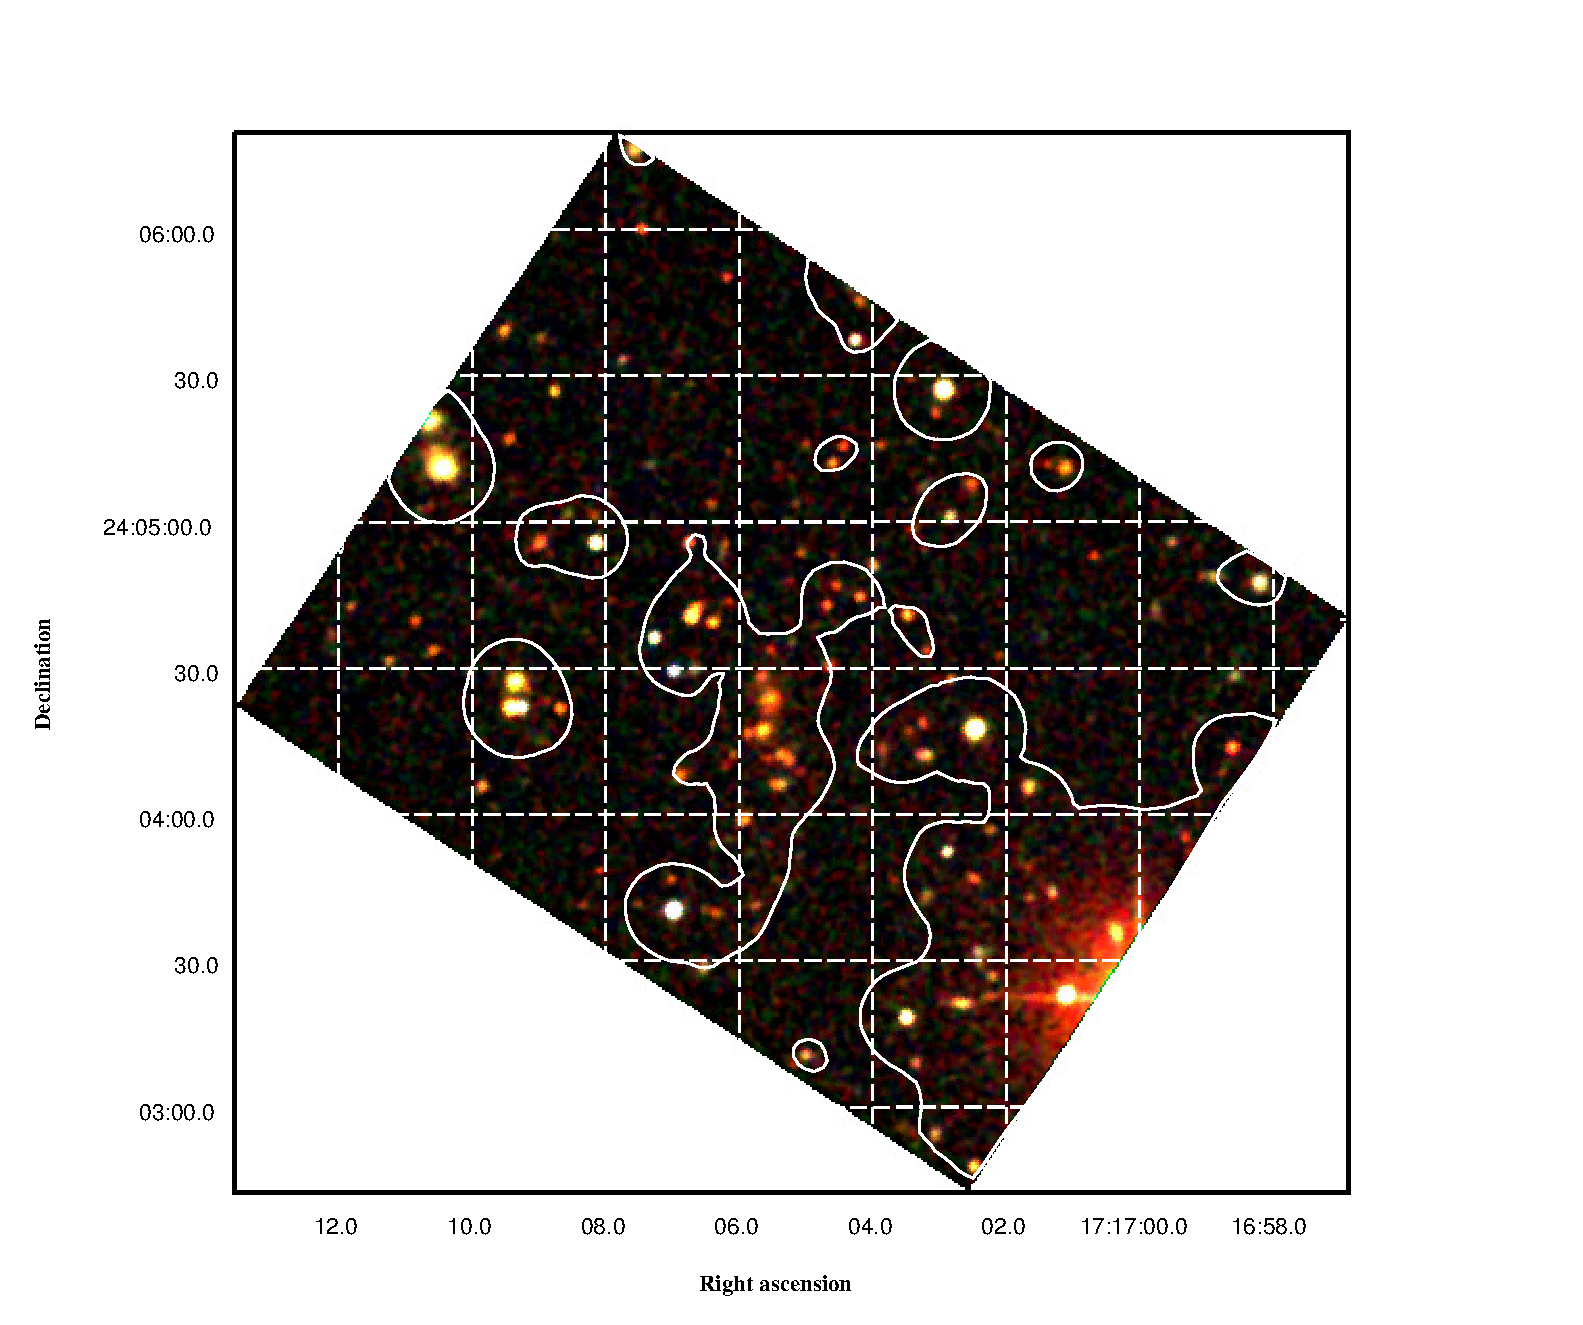
\includegraphics[trim=-0.5cm 0cm 3.5cm 0cm, clip=true, height=6.5cm]{PSZ1G046_SDSS.pdf}
	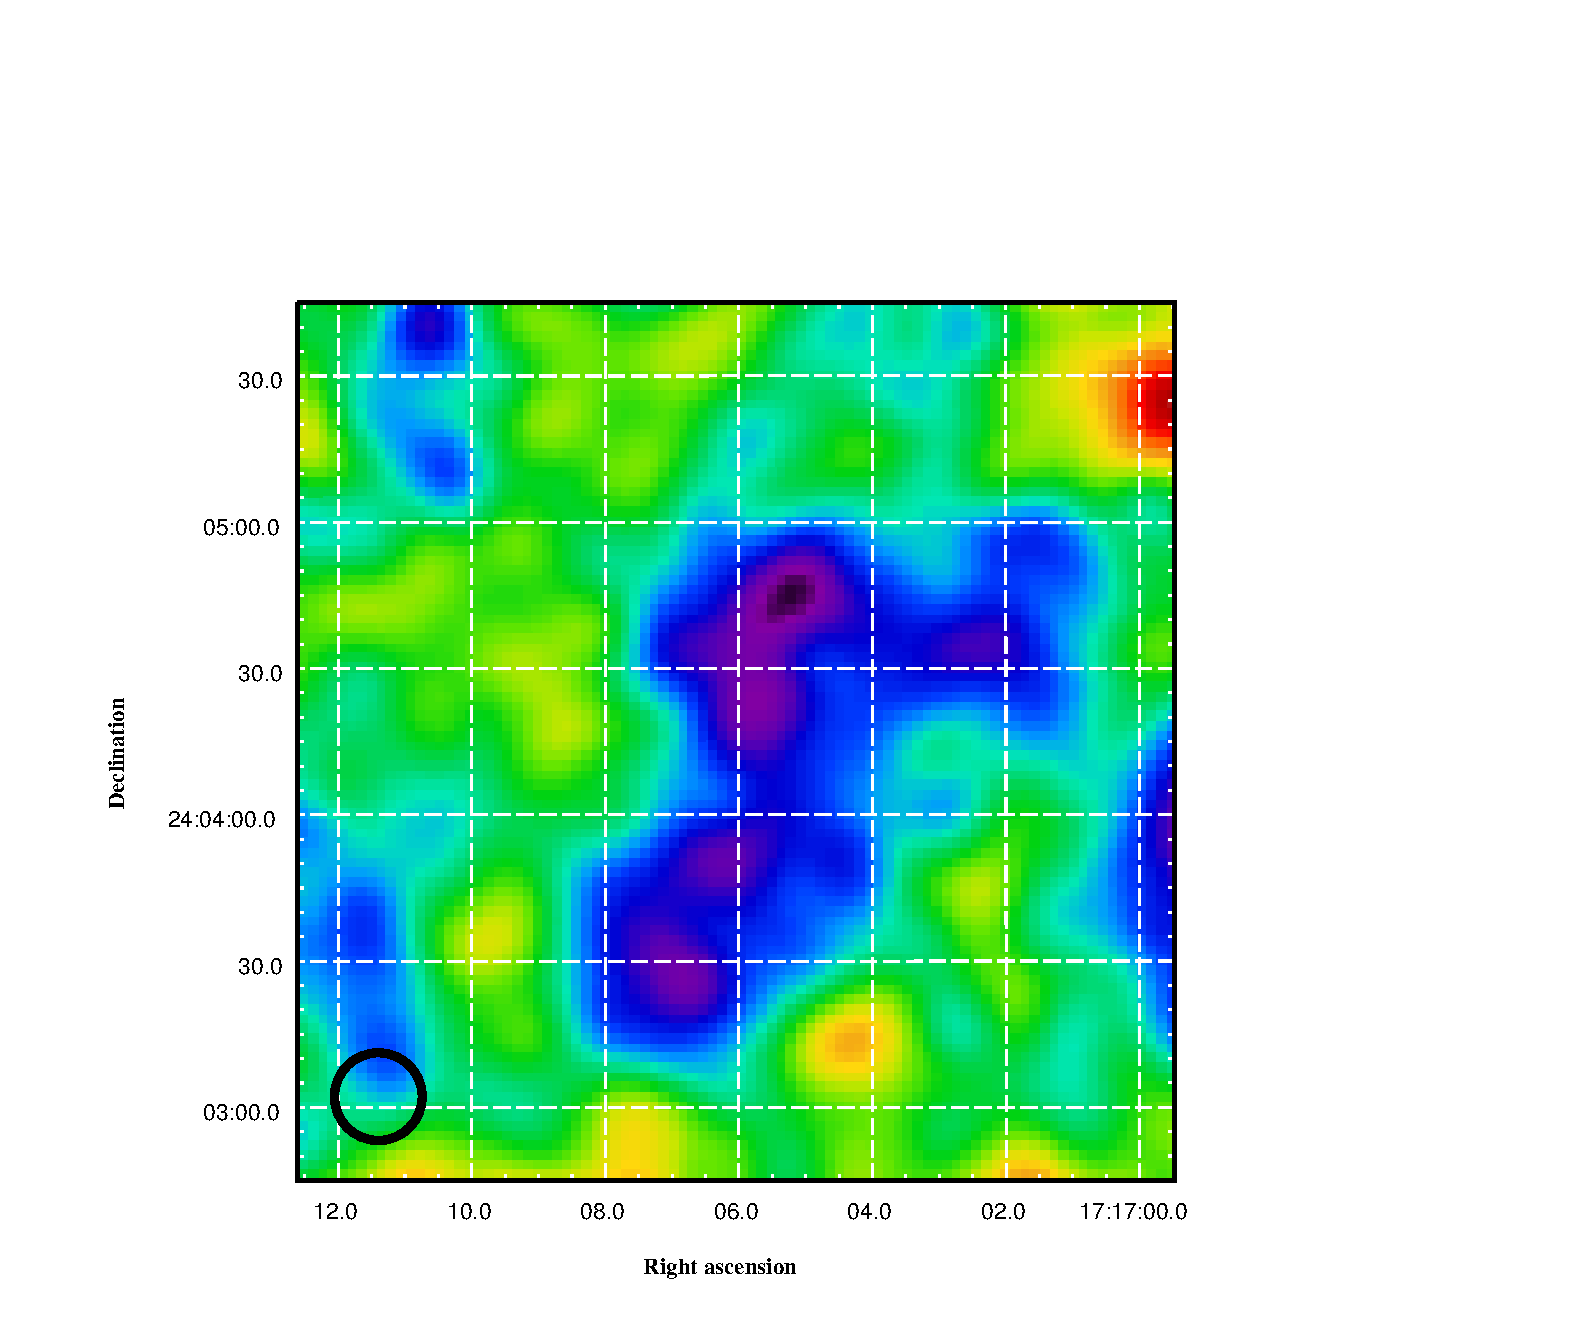
\includegraphics[trim=2.5cm 0cm 6cm 0cm, clip=true,height=6.5cm]{PSZ1G046_NIKA.pdf}
	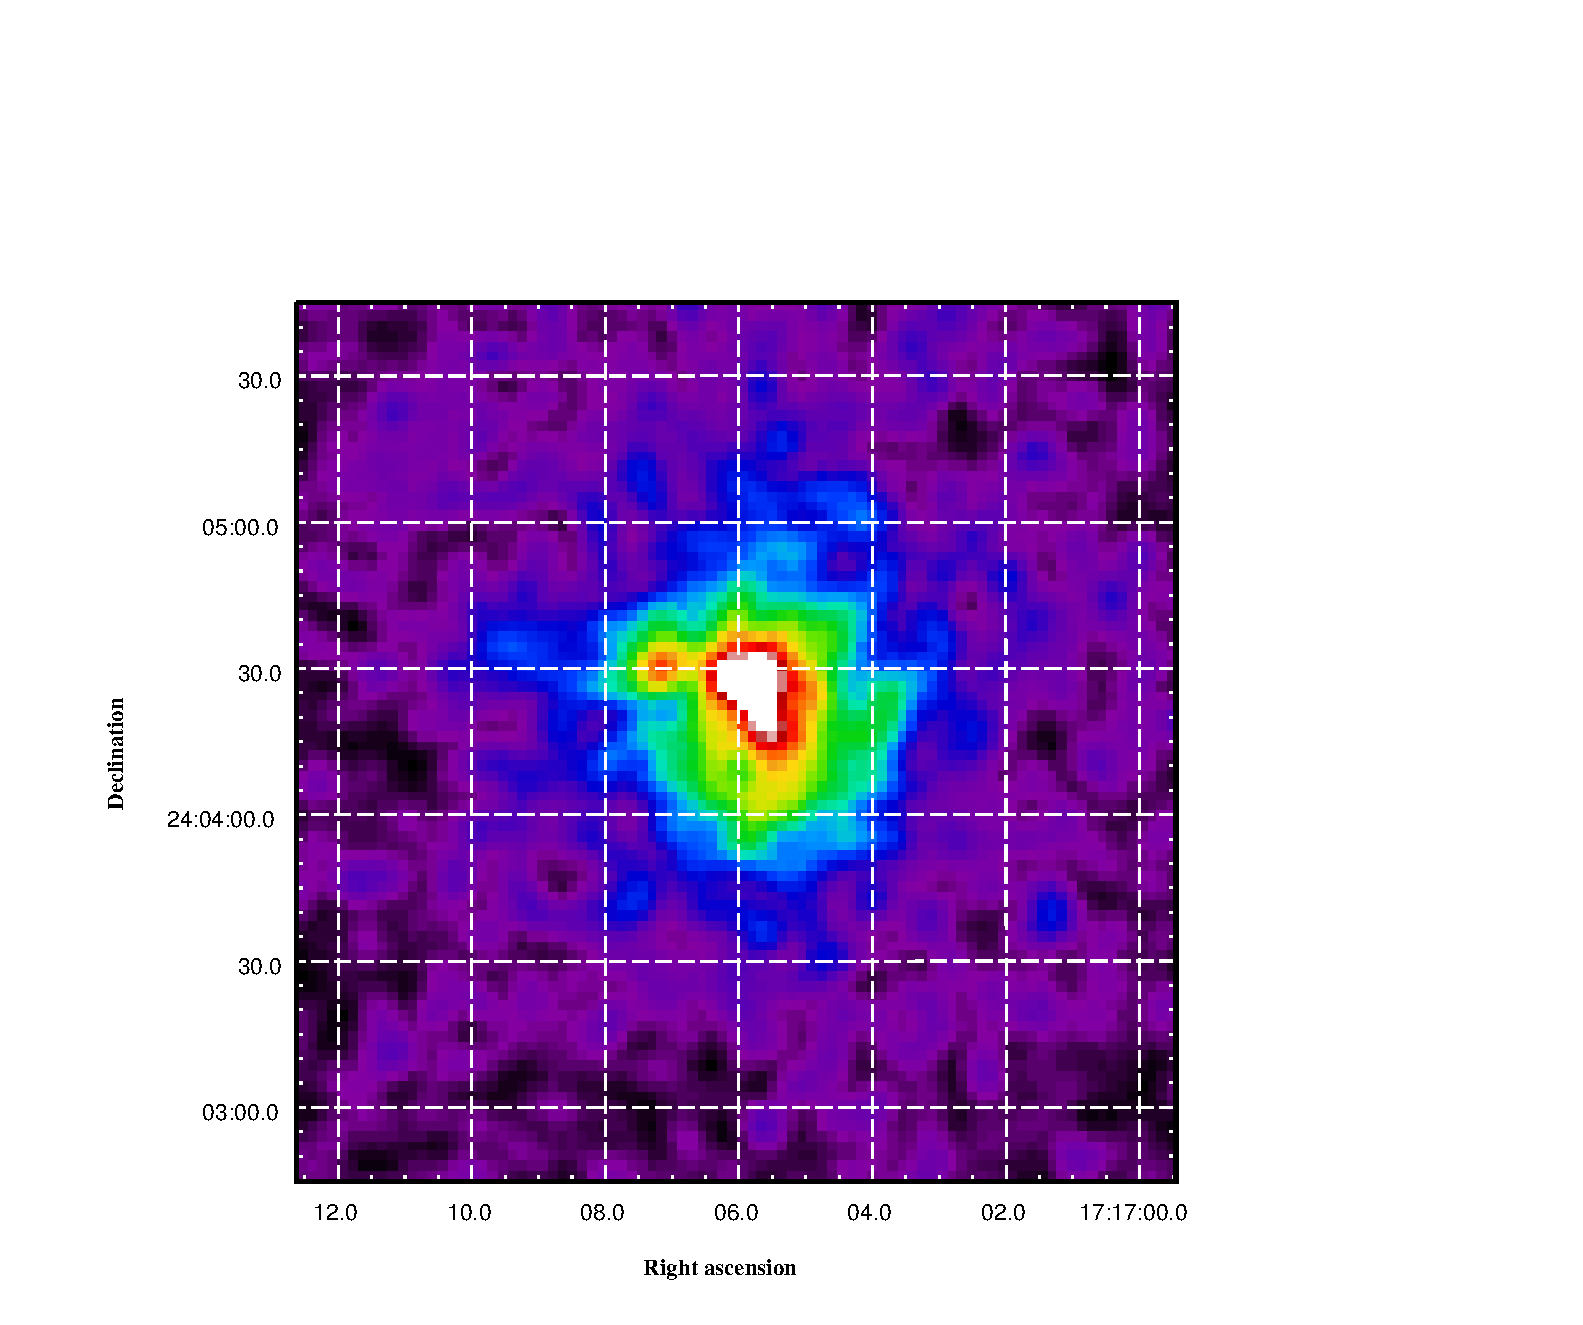
\includegraphics[trim=2.5cm 0cm 6cm 0cm, clip=true,height=6.5cm]{PSZ1G046_XMM.pdf}
	\textbf{PSZ1 G045.85+57.71}\par\medskip
	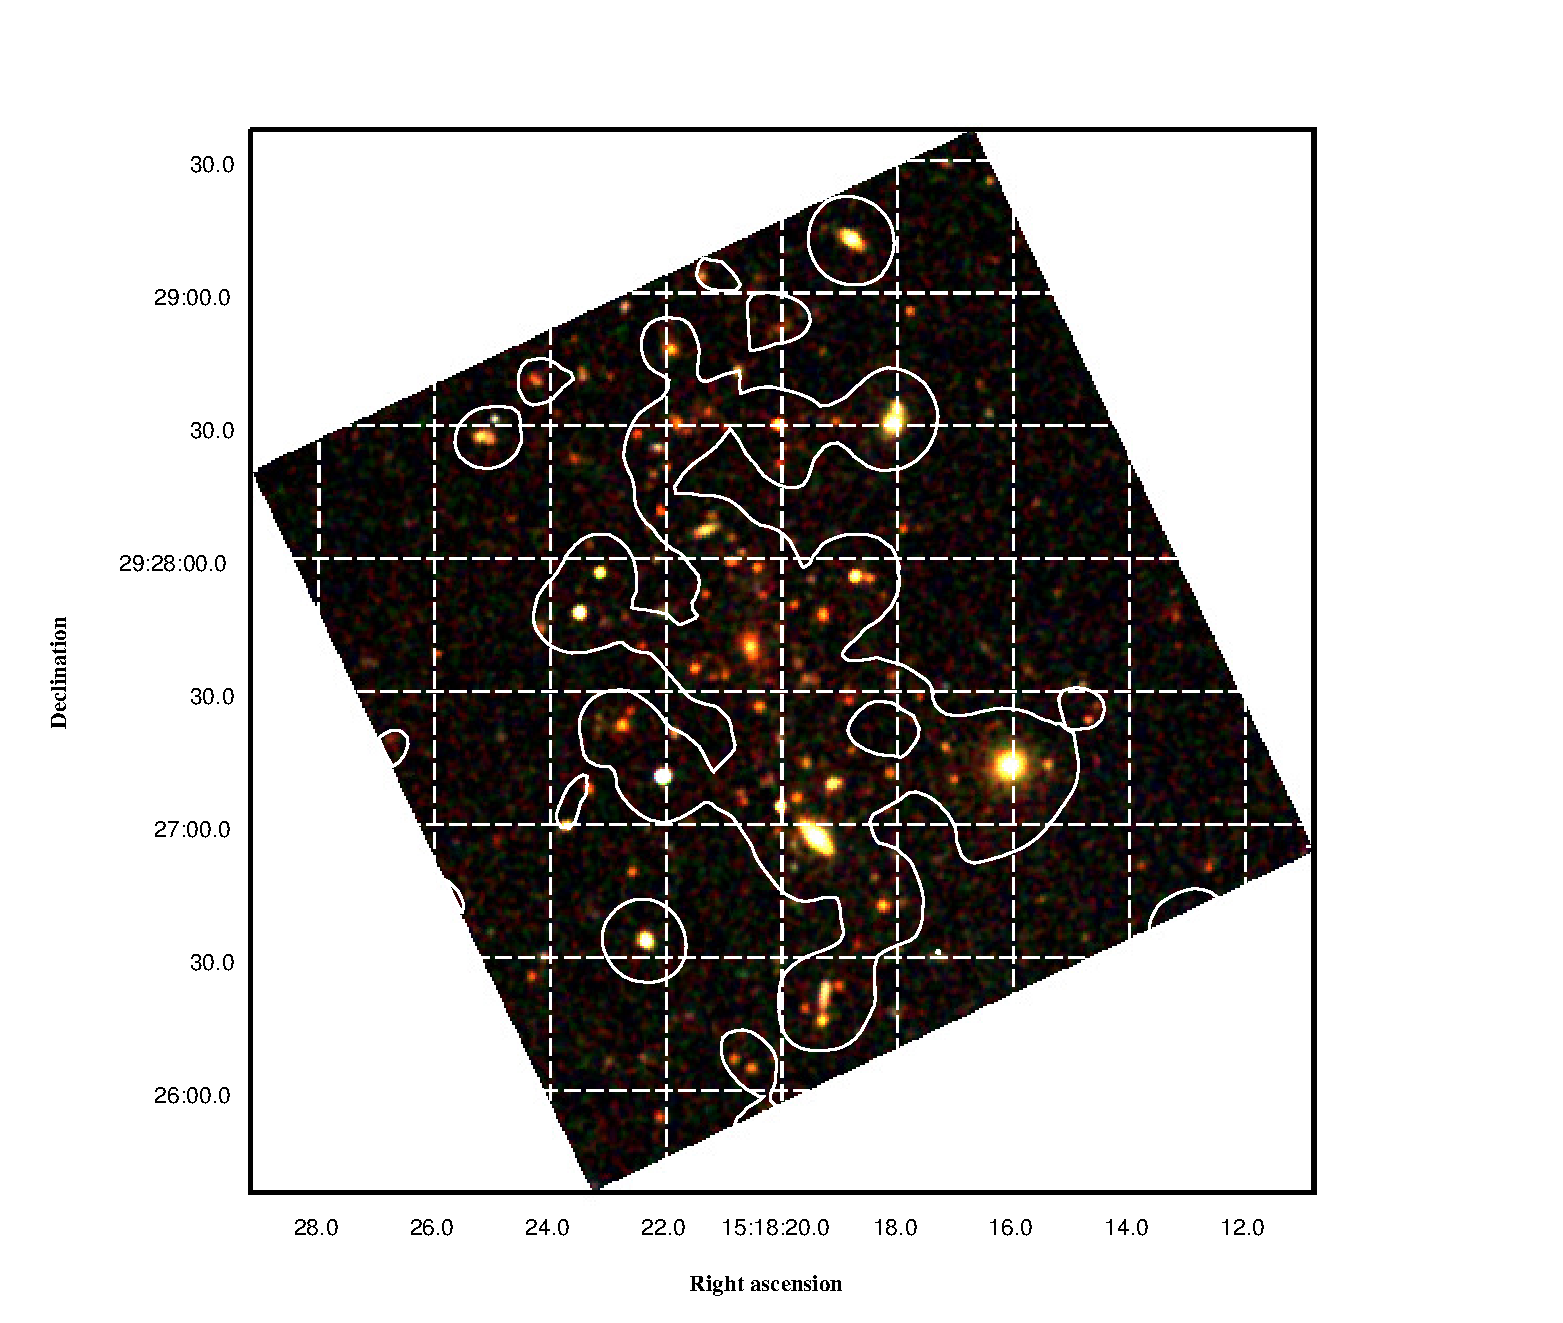
\includegraphics[trim=0.8cm 0cm 3.8cm 0cm, clip=true, height=7.2cm]{PSZ1G045_SDSS.pdf}
	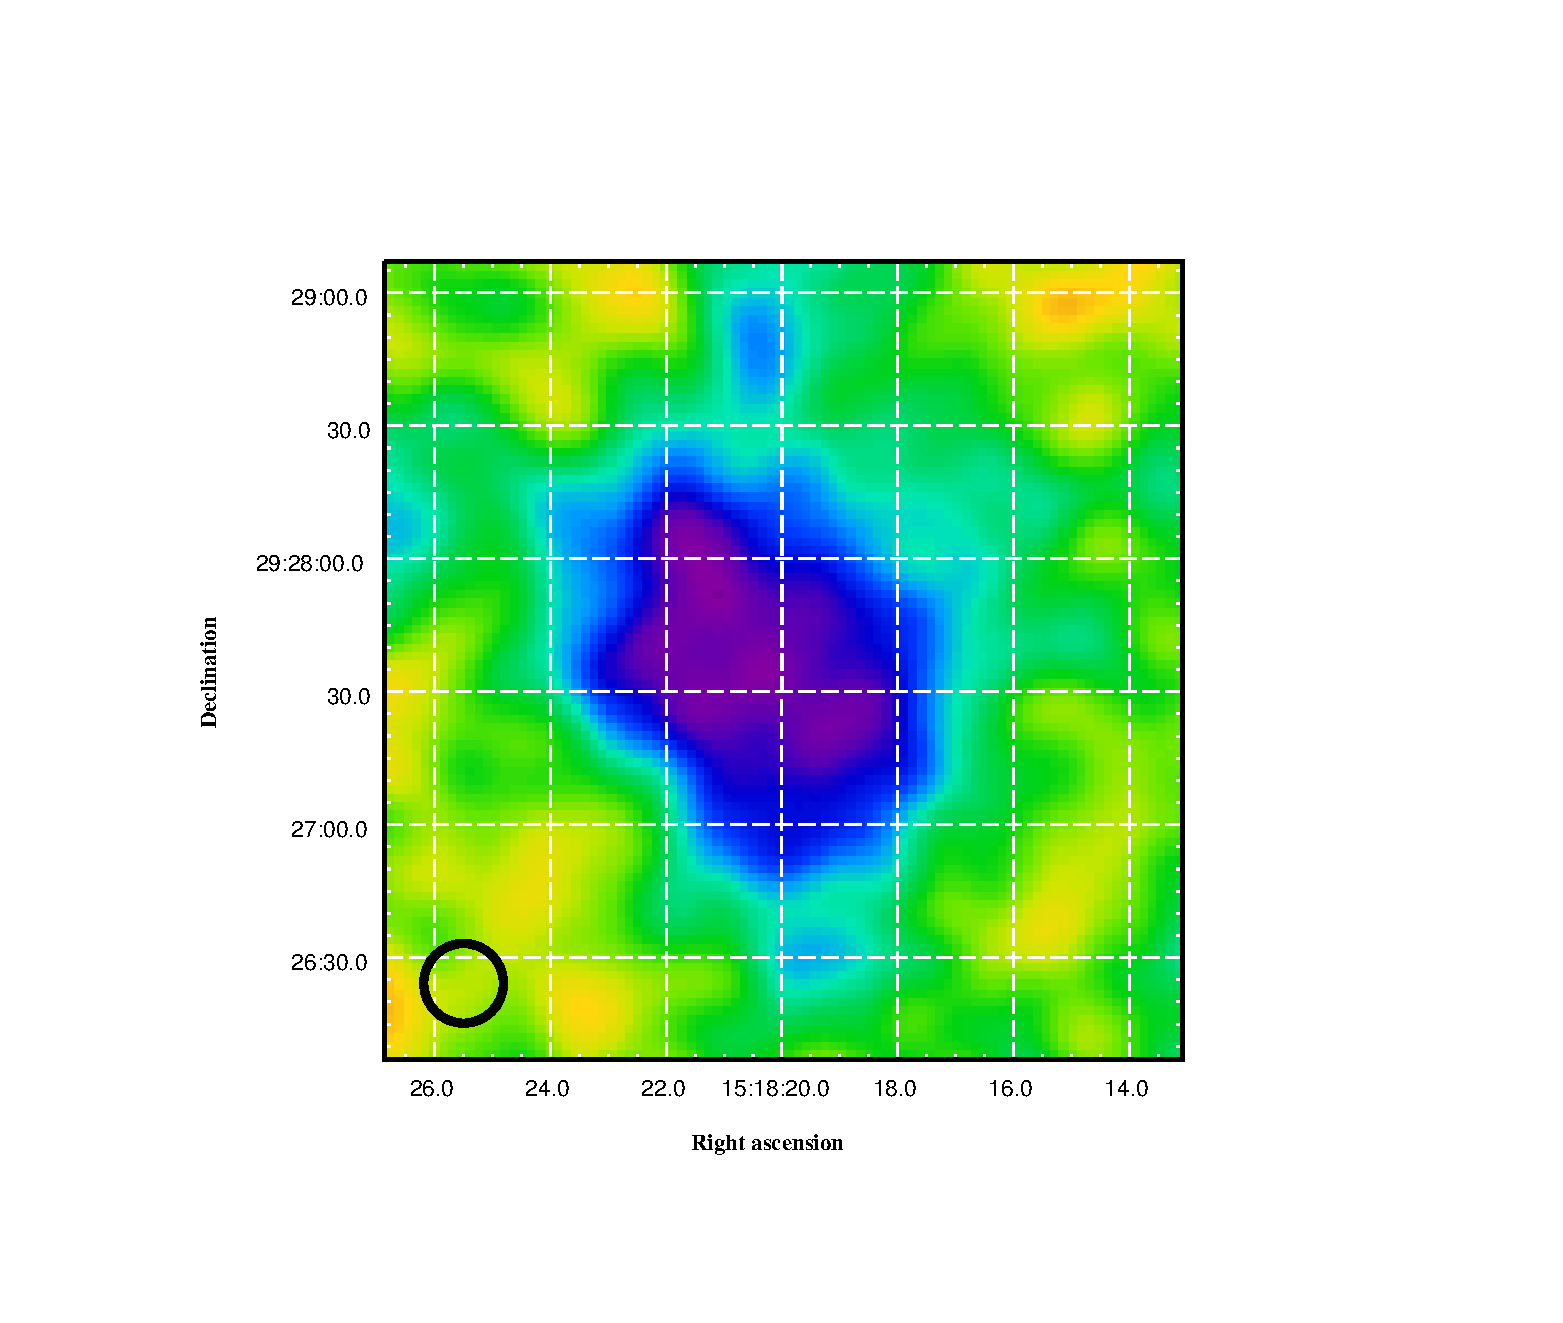
\includegraphics[trim=4.0cm 0cm 6cm 0cm, clip=true,height=7.2cm]{PSZ1G045_NIKA.pdf}
	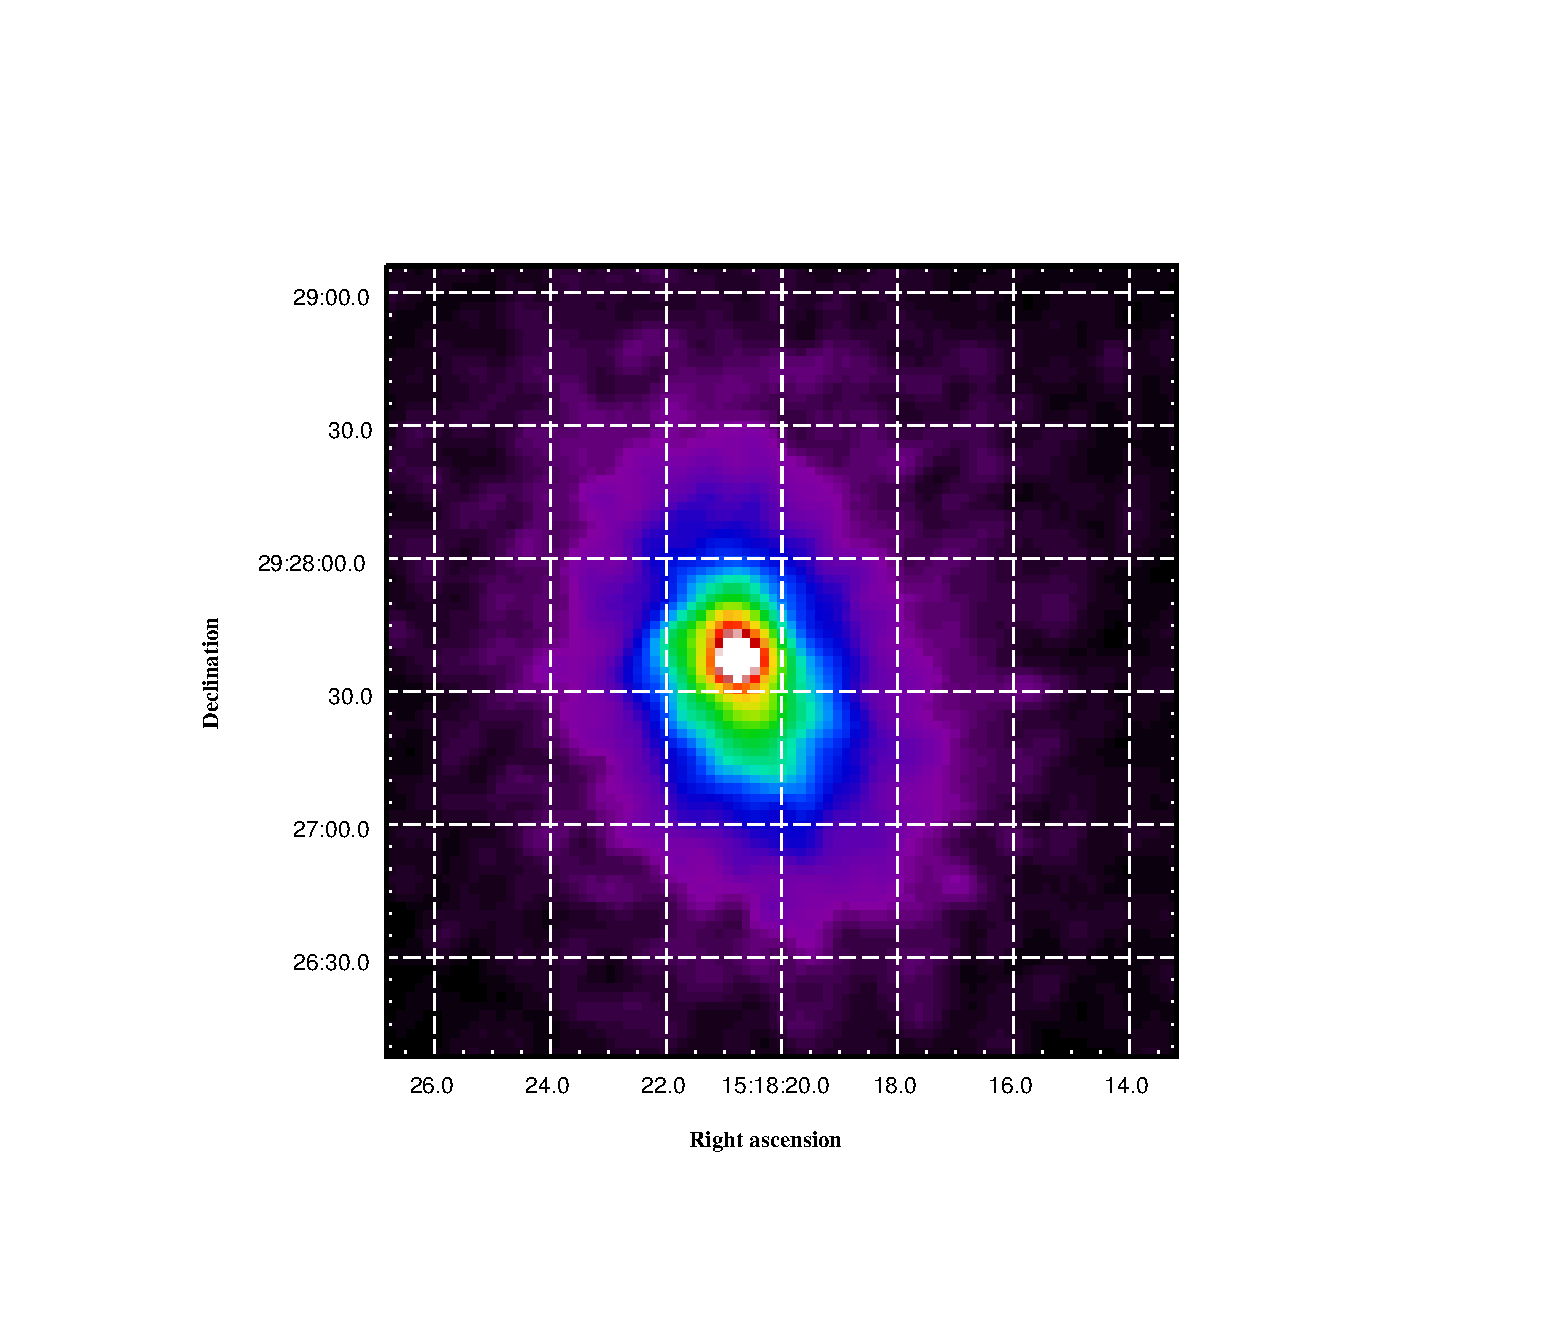
\includegraphics[trim=4.0cm 0cm 6cm 0cm, clip=true,height=7.2cm]{PSZ1G045_XMM.pdf}
	\caption{Matched multi-wavelength comparison of PSZ1 G046.13+30.75 (top) and PSZ1 G045.85+57.71 (bottom). The patches are about 3 $\times$ 3 arcmin$^2$. {\bf Left}: SDSS $i$, $r$, and $g$ bands composite image. The white contours provide a 10 arcsec smoothed brightness distribution in the red band, giving an indication of the cluster galaxy distribution. {\bf Middle}: 18 arcsec resolution NIKA SZ maps at 150~GHz, proportional to the line-of-sight integrated pressure. {\bf Right}: XMM X-ray photon count, roughly proportional to the line-of-sight integrated gas density squared.}
	\label{fig:PSZ1G046} 
\end{figure}

%%%%%%%%%%%%%%%%%%%%%%%%%%%%%%%%%%%%%%%%%%%%%%%%
\begin{thebibliography}{9}

\bibitem[Adam et al. (2015)]{adam2015}
R. Adam, B. Comis, J.-F. MacÌas-PÈrez, {\it et al.}, (2015), A\&A, 576, A12, arXiv:1410.2808

\bibitem[Adam et al. (2014)]{adam2014}
R. Adam, B. Comis, J.-F. MacÌas-PÈrez, {\it et al.}, (2014), A\&A, 569, A66, arXiv:1310.6237

\bibitem[Adam et al. (in preparation)]{adamprep}
R. Adam, B. Comis, I. Bartalucci,  {\it et al.}, in preparation

\bibitem[Allen et al. (2011)]{allen2011}
S. W. Allen, A. E. Evrard, A. B. Mantz, (2011), ARA\&A, 49, 409, arXiv:1103.4829

\bibitem[Calvo et al. (2013)]{calvo2013}
M. Calvo, et al. 2013, A\&A, 551, L12

\bibitem[Catalano et al. (2014)]{catalano2014}
A. Catalano, M. Calvo, N. Ponthieu, {\it et al.}, 2014, A\&A, 569, A9, 1402.0260

\bibitem[Hoekstra et al.(2013)]{hoekstra2013}%Review lensing
H. Hoekstra, M. Bartelmann, H. Dahle {\it et al.} (2013), SSR, 177, 75-118, arXiv:1303.3274

\bibitem[Limousin et al.(2013)]{limousin2013}%Review triaxial
M. Limousin, A. Morandi, M. Sereno {\it et al.}, (2013), SSR, 177, 155-194, arXiv:1210.3067

\bibitem[Monfardini et al. (2011)]{monfardini2011}
A. Monfardini et al. 2011, ApJS, 194, 24, arXiv:102.0870

\bibitem[Monfardini et al. (2010)]{monfardini2010}
A. Monfardini {\it et al.}, 2010, A\&A, 521, A29, arXiv:1004.2209

\bibitem[Morandi et al.(2012)]{morandi2012}%SZ/X/lensing analysis of Abell 1835
A. Morandi, M. Limousin, J. Sayers, {\it et al.} (2012), MNRAS, 425, 2069-2082, arXiv:1111.6189

\bibitem[Planck Collaboration (2015)]{planck_nc_2015}%Planck number count
Planck Collaboration (2015), arXiv:1502.01597

\bibitem[Sembolini et al.(2014)]{sembolini2014}%Baryons in simu
F. Sembolini, M. De Petris, G. Yepes, {\it et al.}, (2014), MNRAS, 440, 3520-3531, arXiv:1309.5387

\end{thebibliography}

\end{document}